\chapter{Evaluation}
\label{sec:results}

The three methods (direct, concurrent indirect and sequential indirect) have been evaluated for bandwidth.
This section presents the results of these evaluations.
All tests were performed 5 times and the results averaged.
In each trial, the memory buffer on the first device was filled with random data.
After the benchmarked transfer from device 1 to device 2, the data was read out from the second device again and compared to the original data to make sure it is correct.

The largest issue that appeared already during the development of the driver is that the direct transfer in the direction from the GPU to the FPGA does not work.
Trying this direction, will make the FPGA board unresponsive or may even result in a complete freeze of the operating system.
This makes the issue hard to debug, because each time a system reboot is required.
Despite extensive efforts, including an analysis of the OpenCL IP system on the FPGA and contacting Altera, this issue could not be fixed during this thesis.



\section{Hardware Configuration}
%stratix v nallatech
%quadro 
%#of pcie lanes
%CPU-Device transfer speed
%driver versions
%amount of memory / type of memory? GDDR?

A NVIDIA Quadro GPU and an Altera Stratix V FPGA were used for the development and evaluation during this thesis.
The relevant features for both devices are shown in the following table:

\begin{center}
\begin{tabular}{| l | c | c |}
	\hline
	 & FPGA \cite{nallatech385} & GPU \cite{quadrok600}\\
	\hline
	\hline
	Model & Nallatech 385-D5 & Hewlett-Packard Quadro K600\\
	\hline
	Architecture & Altera Stratix V D5 & NVIDIA Kepler GK 107\\
	\hline
	Original driver version & 13.1 & 340.58 \\
	\hline
	PCIe Generation & 3.0  & 2.0 \\
	\hline
	Number of PCIe lanes & 8x  & 16x \\
	\hline
	Global memory size & 8GB  & 1GB \\
	\hline
	Memory type & DDR3  & GDDR3 \\
	\hline
	Measured bandwidth to CPU & 750 MB/s & 1930 MB/s\\
	\hline
	Measured bandwidth from CPU & 550 MB/s & 1950 MB/s\\
	\hline
\end{tabular}
\end{center}




\section{Effects of RDMA Optimizations} 

To  find out to which extent the optimizations from section \ref{sec:optimizations} contribute to the final performance, each of them has been evaluated.
The results are shown in figure \ref{fig:optimizations_eval}.

The first version, that was developed mainly as a prototype performs very poorly, as expected.
A maximum bandwidth of only 170 MB/s has been measured, which is even slower than the sequential indirect transfer method.
Its main bottleneck is the response latency from a PCIe interrupt until the next descriptor is sent, as indicated by the measurements from the larger descriptors optimization.
This optimization had the largest impact, raising the bandwidth to ca. 580 MB/s for large transfers with 512KB descriptor sizes.


The multiple descriptors optimization raises the maximum measured bandwidth to ca. 610 MB/s.
The overall improvement is rather small because of the limitation of being able to process only 2 descriptors at a time which in turn is due to the small ATT.

Lazy unpinning contributes a roughly constant performance gain, independent of the transfer size.
This is especially important for the smaller transfers.
Note that the data for this version does not include the first transfer, which performs the actual pinning and does not benefit from this optimization.
Only the subsequent transfers are considered.
This is nevertheless representable, since real applications usually require many transfers.

\begin{figure}[htb]
	  \centerline{
		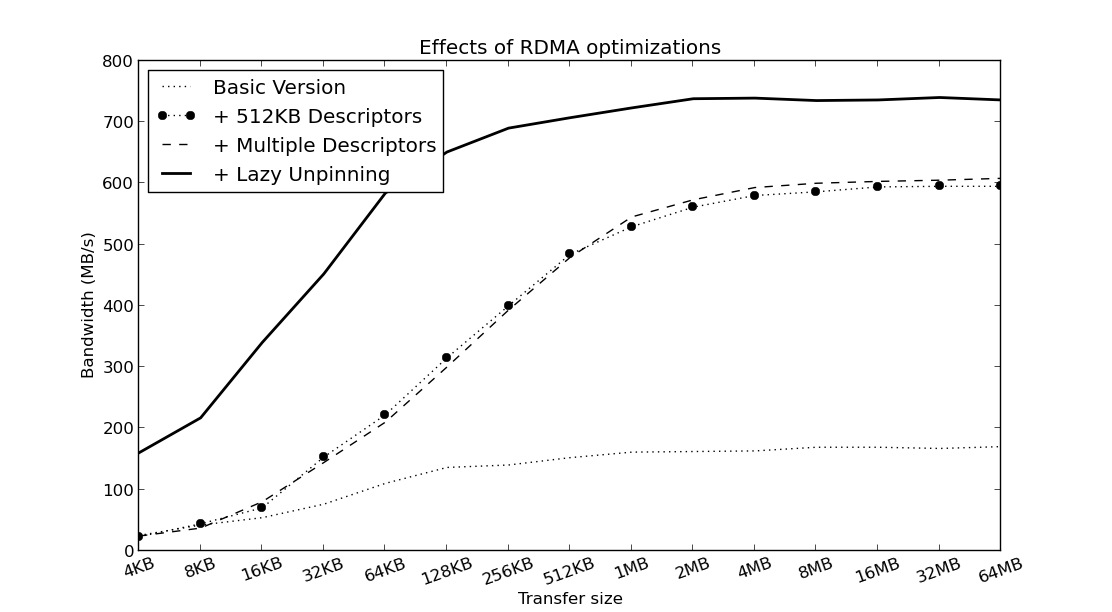
\includegraphics[width=1.3\textwidth]{images/optimizations_eval2}}
	  \caption{Comparison of the optimizations described in section \ref{sec:optimizations}. Each optimization is added to the previous version (i.e. the Lazy Unpinning benchmark also includes the Multiple Descriptors and 512KB Descriptors optimizations). The Lazy Unpinning benchmark does not include the first transfer, which performs the actual memory pinning.}
	  \label{fig:optimizations_eval}
\end{figure}


\section{Parameter Choice for Concurrent Indirect Transfer}
\label{sec:results_concurrent}

As already mentioned in section \ref{section:concurrent}, the choice of the block size parameter is important for the concurrent indirect transfer method.
Different values have been evaluated. Figure \ref{fig:results_blocksizes} presents the results.

The preliminary idea that too small and too large block sizes are detrimental can be confirmed.
However, the extent partly depends on the transfer size and direction.
For the direction from the GPU to the FPGA, a block size of one fourth of the transfer size seems to be an overall good choice.
The opposite direction is not as clear.
Large transfers seem to benefit from smaller block sizes of ca. one eighth of the overall size, whereas for small transfers the synchronization costs are rather large and a blocks of one half of the overall size should be chosen.


\begin{figure}[h]
\begin{center}$
\begin{array}{cc}
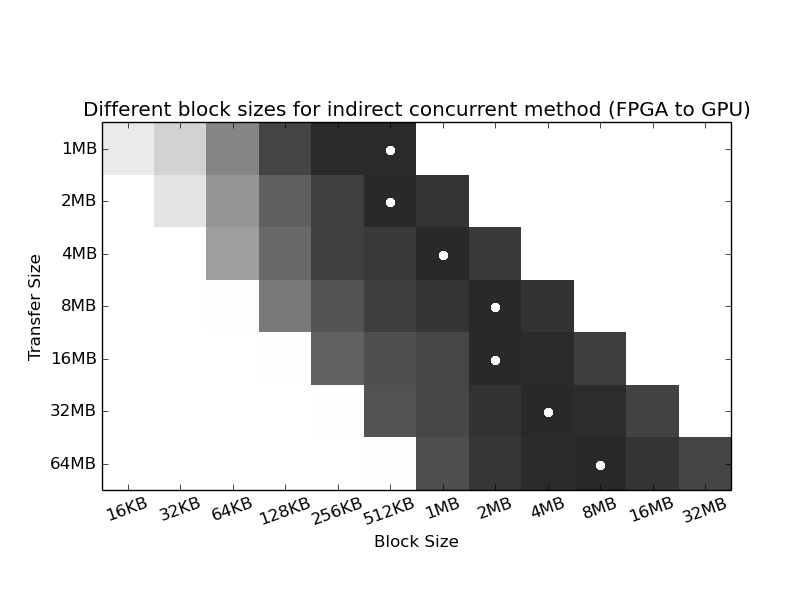
\includegraphics[height=0.45\textheight]{images/fg_dots.png} \\
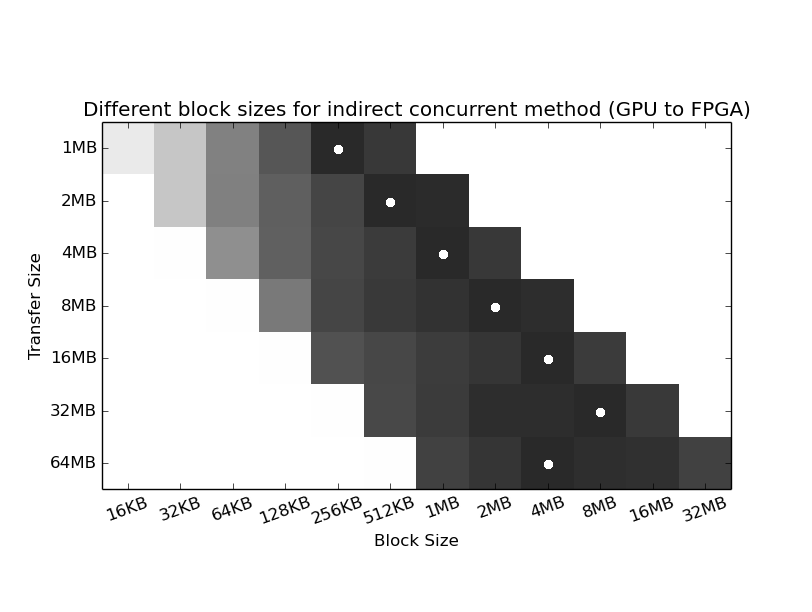
\includegraphics[height=0.45\textheight]{images/gf_dots.png}
\end{array}$
\end{center}
\caption{Influence of the block size parameter on the performance for the concurrent indirect transfer method. Higher bandwidth is darker. The white dots mark the maximum bandwidth for each transfer.}
\label{fig:results_blocksizes}
\end{figure}


%TODO: bar plot of five transfers that shows lazy unpinning effect?



\section{Method Comparison}

Figure \ref{fig:results_comparison} presents a comparison of the sequential indirect, concurrent indirect and the direct transfer methods.
For contrast, the CPU-FPGA bandwidth, which can be regarded as an upper limit for the GPU-FPGA bandwidth, is also shown.
Again, the first transfer which includes the expensive pinning operation is not included in the graphs.

Different block size values were used for the concurrent indirect method:
Transfers with sizes until including 1MB used a value of one half, from 2MB until 8MB a value of one fourth and from 16MB on a value of one eighth  of the overall size.

As expected, the direct transfer method is indeed the fastest of the three methods, peaking at 740MB/s.
For large transfers the concurrent indirect approach performs almost as well with a speed of up to 730MB/s.
This results in a speed-up of ca 30\% and 28\% compared with the indirect transfers.
For the direction from the GPU to the FPGA, for which the direct transfer could not be enabled, this is even the best solution, with a bandwidth of ca 525MB/s and a speed-up of ca 39\%.



The bandwidth of the direct method deteriorates after the 192MB transfer size mark.
This is due to the limitation of the graphics card not being able to pin more than ca. 200MB at a time.
For larger transfers, a memory region has to be unpinned first which costs a significant amount of time.

The 512MB transfer for the concurrent indirect method failed to succeed.
Presumably, the pinned CPU memory buffer (mentioned in section \ref{section:concurrent}) uses up space not only on the CPU but also on the GPU.
As a consequence this exceeds the memory limit of the Quadro K600 of 1GB.


%first transfer not included because of pinning


\begin{figure}[h]
\begin{center}
$
\begin{array}{cc}
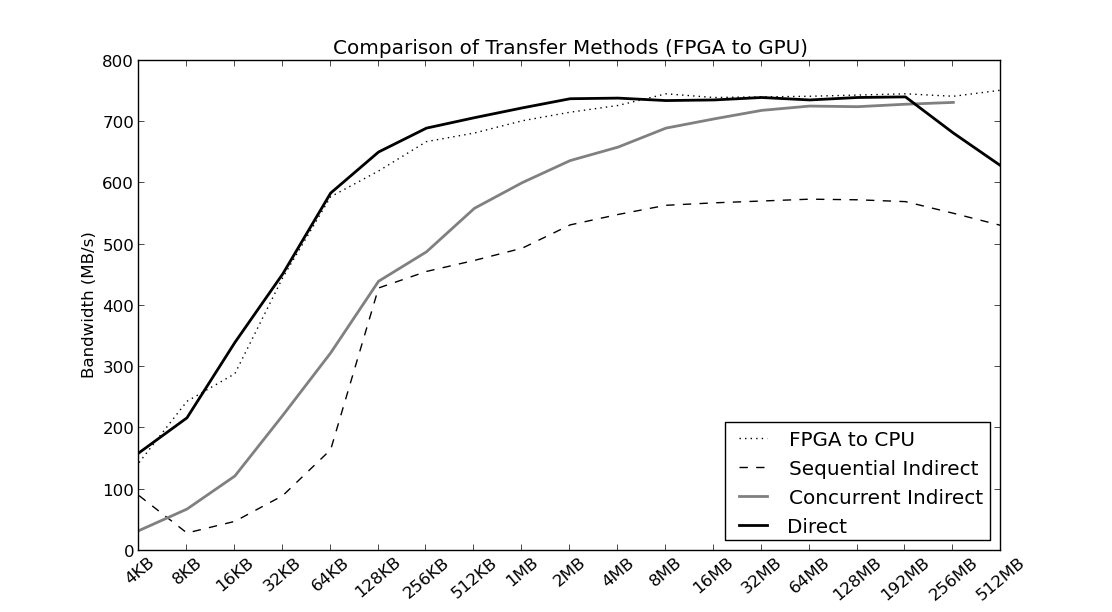
\includegraphics[height=0.41\textheight]{images/results_comp1.png} \\
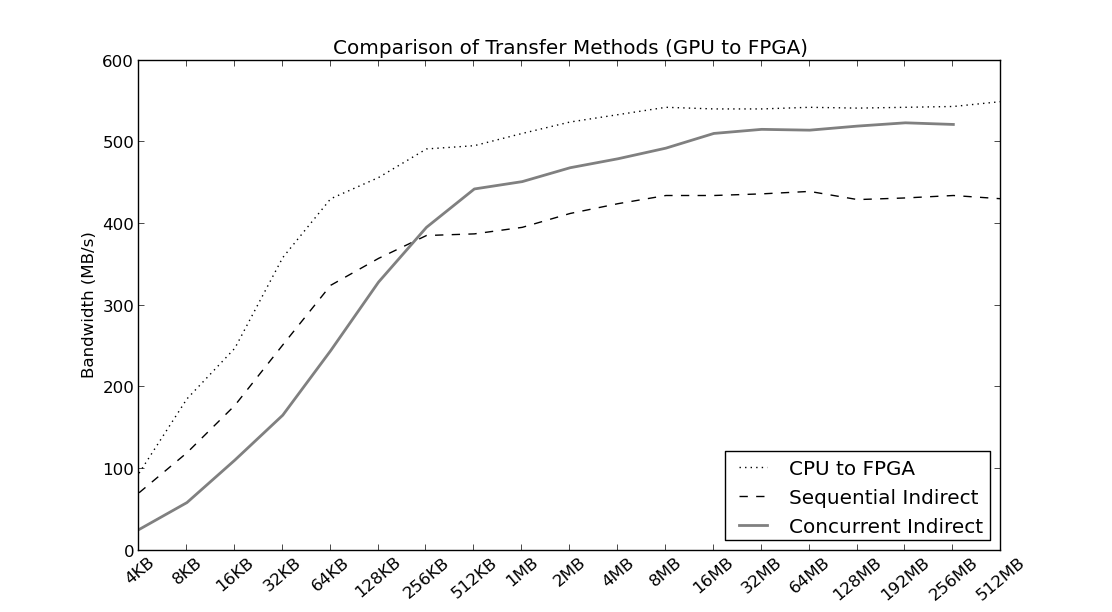
\includegraphics[height=0.41\textheight]{images/results_comp2.png}
\end{array}
$
\end{center}
\caption{Comparison of sequential indirect, concurrent indirect and direct transfer methods.}
\label{fig:results_comparison}
\end{figure}




\section{Comparison with Previous Work}
\label{section:previousworkcomparison}

The following table compares the relevant features of the approaches from previous research, presented in section \ref{section:previouswork} and the two approaches from this thesis, direct and concurrent indirect (the two columns on the right).
Note that the bandwidths cannot be simply compared due to different devices.


\begin{center}
\begin{tabular}{| l || c| c |c|| c | c |}
	\hline
		&	\multicolumn{3}{c||}{Previous Work} & \multicolumn{2}{c|}{This Thesis}\\
	\hline
		&	Bittner \& Ruf & FPGA$^2$ & Susanto & Direct & Concurrent\\
	\hline\hline
	Operating System & Windows & Linux & Linux & \multicolumn{2}{c|}{Linux}\\
	\hline
	DMA Master & GPU & FPGA & FPGA & FPGA & Both \\
	\hline
	Processes & 1 & 1 & 2 & \multicolumn{2}{c|}{1}\\
	\hline
	FPGA Vendor & Xilinx & Xilinx & Altera & \multicolumn{2}{c|}{Altera}\\
	\hline
	FPGA Model & Virtex 6 & Virtex 5 & Stratix V & \multicolumn{2}{c|}{Stratix V}\\
	\hline
	FPGA IP Stack & Custom & Custom & Vendor & \multicolumn{2}{c|}{Vendor} \\
	\hline
	FPGA Driver & Custom & Custom & Modified & Modified & Original\\
	\hline
	FPGA Programming & HDL & HDL & OpenCL & \multicolumn{2}{c|}{OpenCL}\\
	\hline
	GPU Vendor & NVIDIA & NVIDIA & NVIDIA & \multicolumn{2}{c|}{NVIDIA}\\
	\hline
	GPU Model & GeForce& GeForce & GeForce & \multicolumn{2}{c|}{Quadro}\\
	&  GTX580 & 8400GS & GTX660Ti &  \multicolumn{2}{c|}{K600}\\
	\hline
	GPU Driver & Original & Nouveau & Original & Modified & Original \\
	\hline
	GPU Programming & CUDA & gdev & CUDA & \multicolumn{2}{c|}{OpenCL}\\
	\hline
	Effective PCIe lanes & 8 & 1 & 8 & \multicolumn{2}{c|}{8}\\
	\hline
	Effective & 1.0 & 1.1 & not & \multicolumn{2}{c|}{2.0}\\
	PCIe generation & & & specified & \multicolumn{2}{c|}{} \\
	\hline
	\hline
	Maximal bandwidth & 514MB/s & 203MB/s & 680MB/s & 740MB/s & 730MB/s\\
	FPGA to GPU & & & & &\\
	\hline
	Maximal bandwidth & 1.6GB/s & 189MB/s & 540MB/s & N/A & 525MB/s\\
	GPU to FPGA & & & & &\\
	\hline
\end{tabular}
\end{center}

The approaches that utilize the FPGA as the DMA master perform better for the direction from the FPGA to the GPU.
The opposite is true if the GPU is used as the DMA master.
This may have to do with the PCIe protocol: an extra PCIe packet is required to read from another device, whereas writing to the other device requires only one packet.



